\documentclass[compress]{beamer}
\usepackage{ifthen,verbatim}

%% \title{PUT_TITLE_HERE}
%% \author{Jim Pivarski, Alexei Safonov, K\'aroly Banicz$^*$}
%% \institute{Texas A\&M University, $^*$FermiLab}
%% \date{22 April, 2008}

\newcommand{\isnote}{}
\xdefinecolor{lightyellow}{rgb}{1.,1.,0.25}
\xdefinecolor{darkblue}{rgb}{0.1,0.1,0.7}

%% Uncomment this to get annotations
%% \def\notes{\addtocounter{page}{-1}
%%            \renewcommand{\isnote}{*}
%% 	   \beamertemplateshadingbackground{lightyellow}{white}
%%            \begin{frame}
%%            \frametitle{Notes for the previous page (page \insertpagenumber)}
%%            \itemize}
%% \def\endnotes{\enditemize
%% 	      \end{frame}
%%               \beamertemplateshadingbackground{white}{white}
%%               \renewcommand{\isnote}{}}

%% Uncomment this to not get annotations
\def\notes{\comment}
\def\endnotes{\endcomment}

\setbeamertemplate{navigation symbols}{}
\setbeamertemplate{headline}{\mbox{ } \hfill
\begin{minipage}{5.5 cm}
\vspace{-0.75 cm} \small
\end{minipage} \hfill
\begin{minipage}{4.5 cm}
\vspace{-0.75 cm} \small
\begin{flushright}
\ifthenelse{\equal{\insertpagenumber}{1}}{}{Jim Pivarski \hspace{0.2 cm} \insertpagenumber\isnote/\pageref{numpages}}
\end{flushright}
\end{minipage}\mbox{\hspace{0.2 cm}}\includegraphics[height=1 cm]{../cmslogo} \hspace{0.1 cm} \includegraphics[height=1 cm]{../tamulogo} \hspace{0.01 cm} \vspace{-1.05 cm}}

\begin{document}
% \frame{\titlepage}

%% \begin{notes}
%% \item This is the annotated version of my talk.
%% \item If you want the version that I am presenting, download the one
%% labeled ``slides'' on Indico (or just ignore these yellow pages).
%% \item The annotated version is provided for extra detail and a written
%% record of comments that I intend to make orally.
%% \item Yellow notes refer to the content on the {\it previous} page.
%% \item All other slides are identical for the two versions.
%% \end{notes}

\begin{frame}
\frametitle{Using the even-odd procedure\ldots}
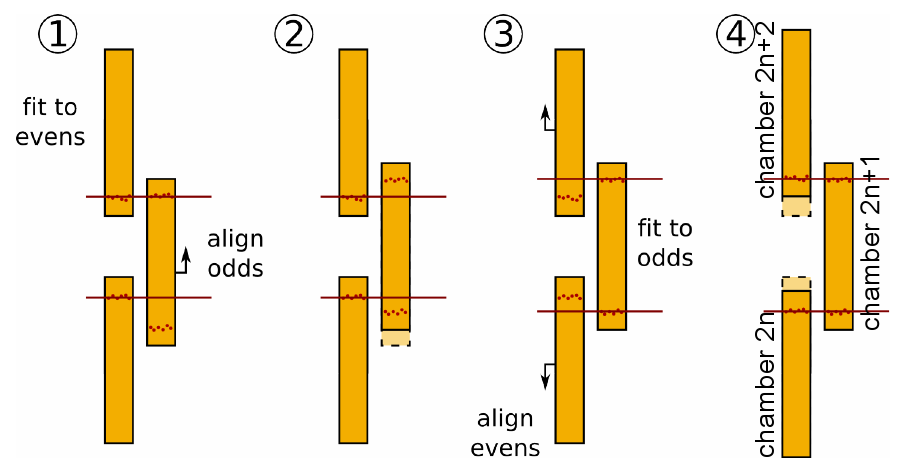
\includegraphics[width=\linewidth]{even-odd.png}

\vfill
\small (In ME+2/1 with 1000 high-momentum tracks after overlap-selection)
\end{frame}

\begin{frame}
\frametitle{Local \only<1-4>{$x$}\only<5>{$y$}\only<6>{$\phi_y$}\only<7>{$\phi_z$} alignment}

\begin{center}
\only<1>{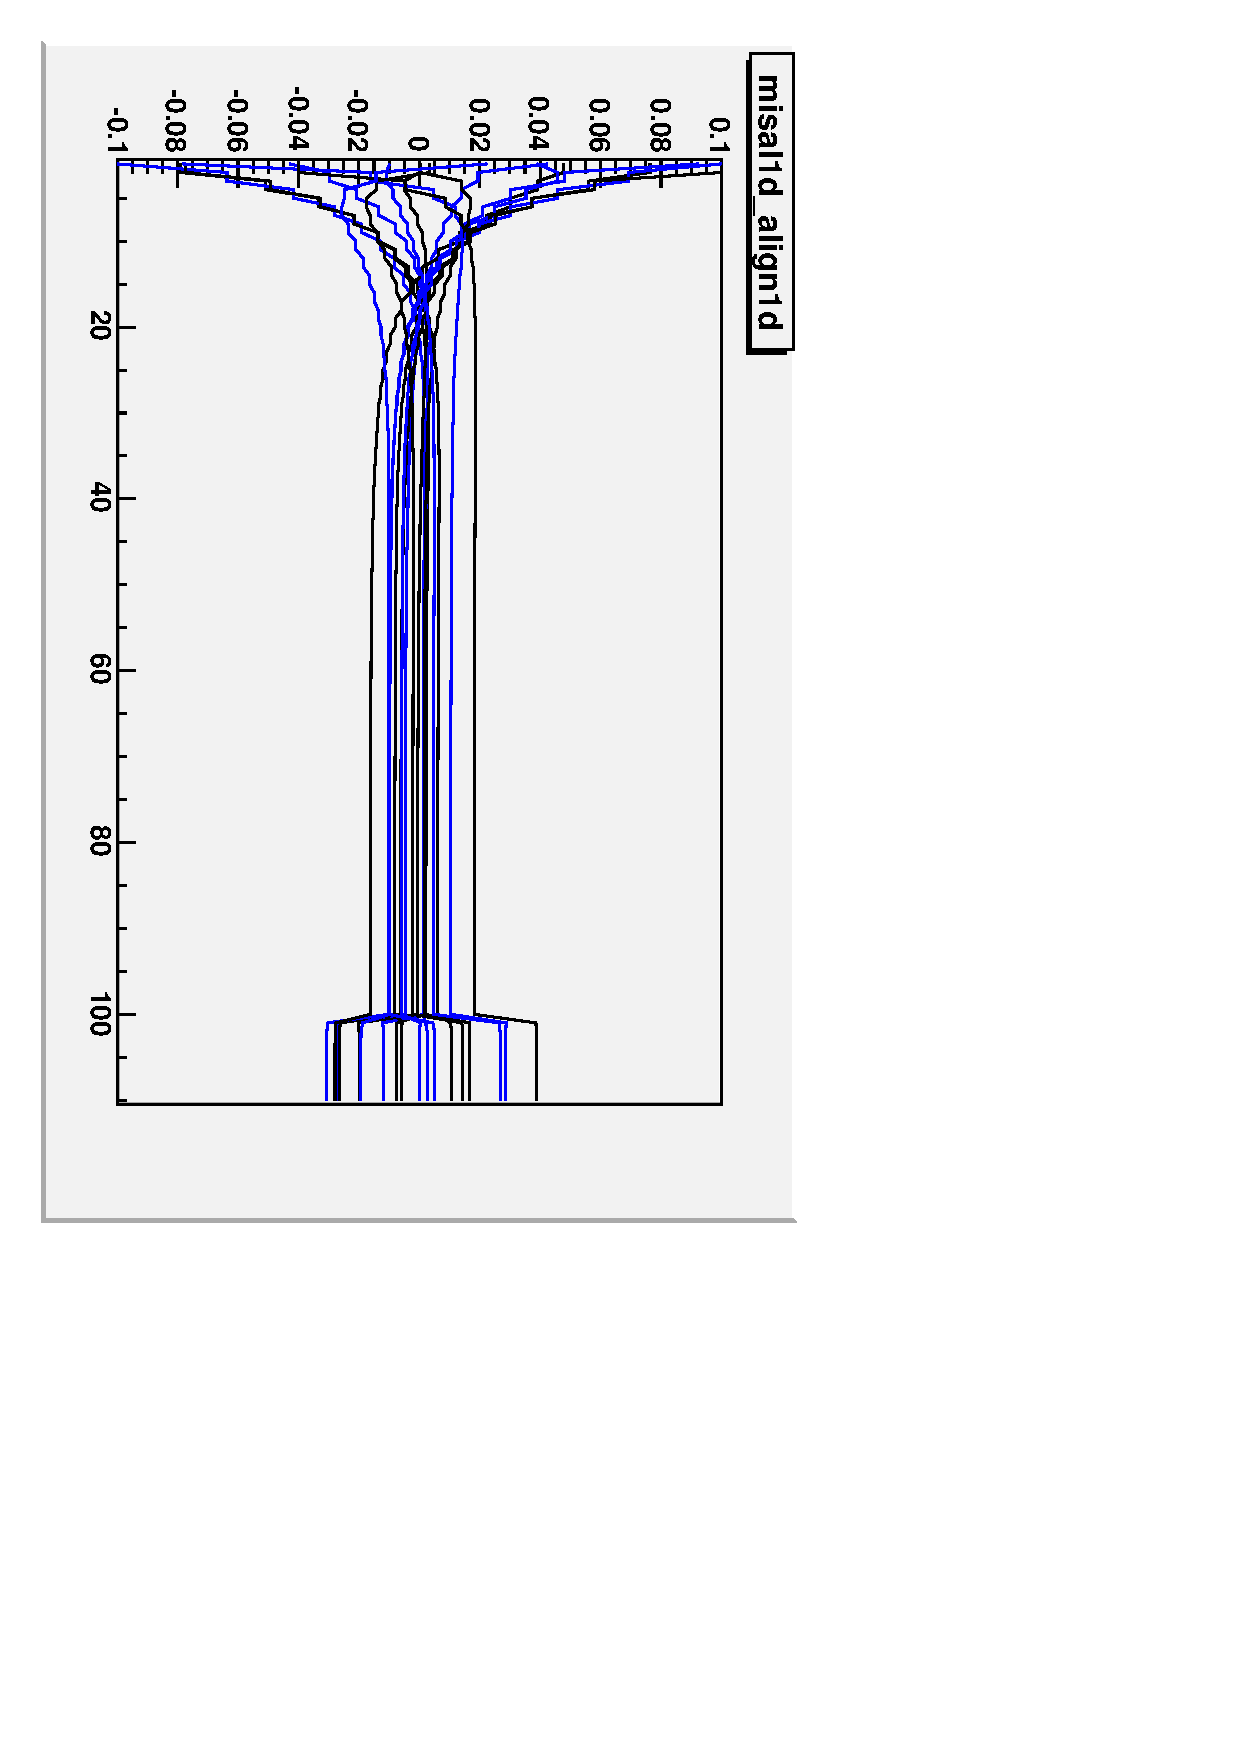
\includegraphics[height=0.9\linewidth, angle=90]{misal1d_align1d_lookx.pdf}}
\only<2>{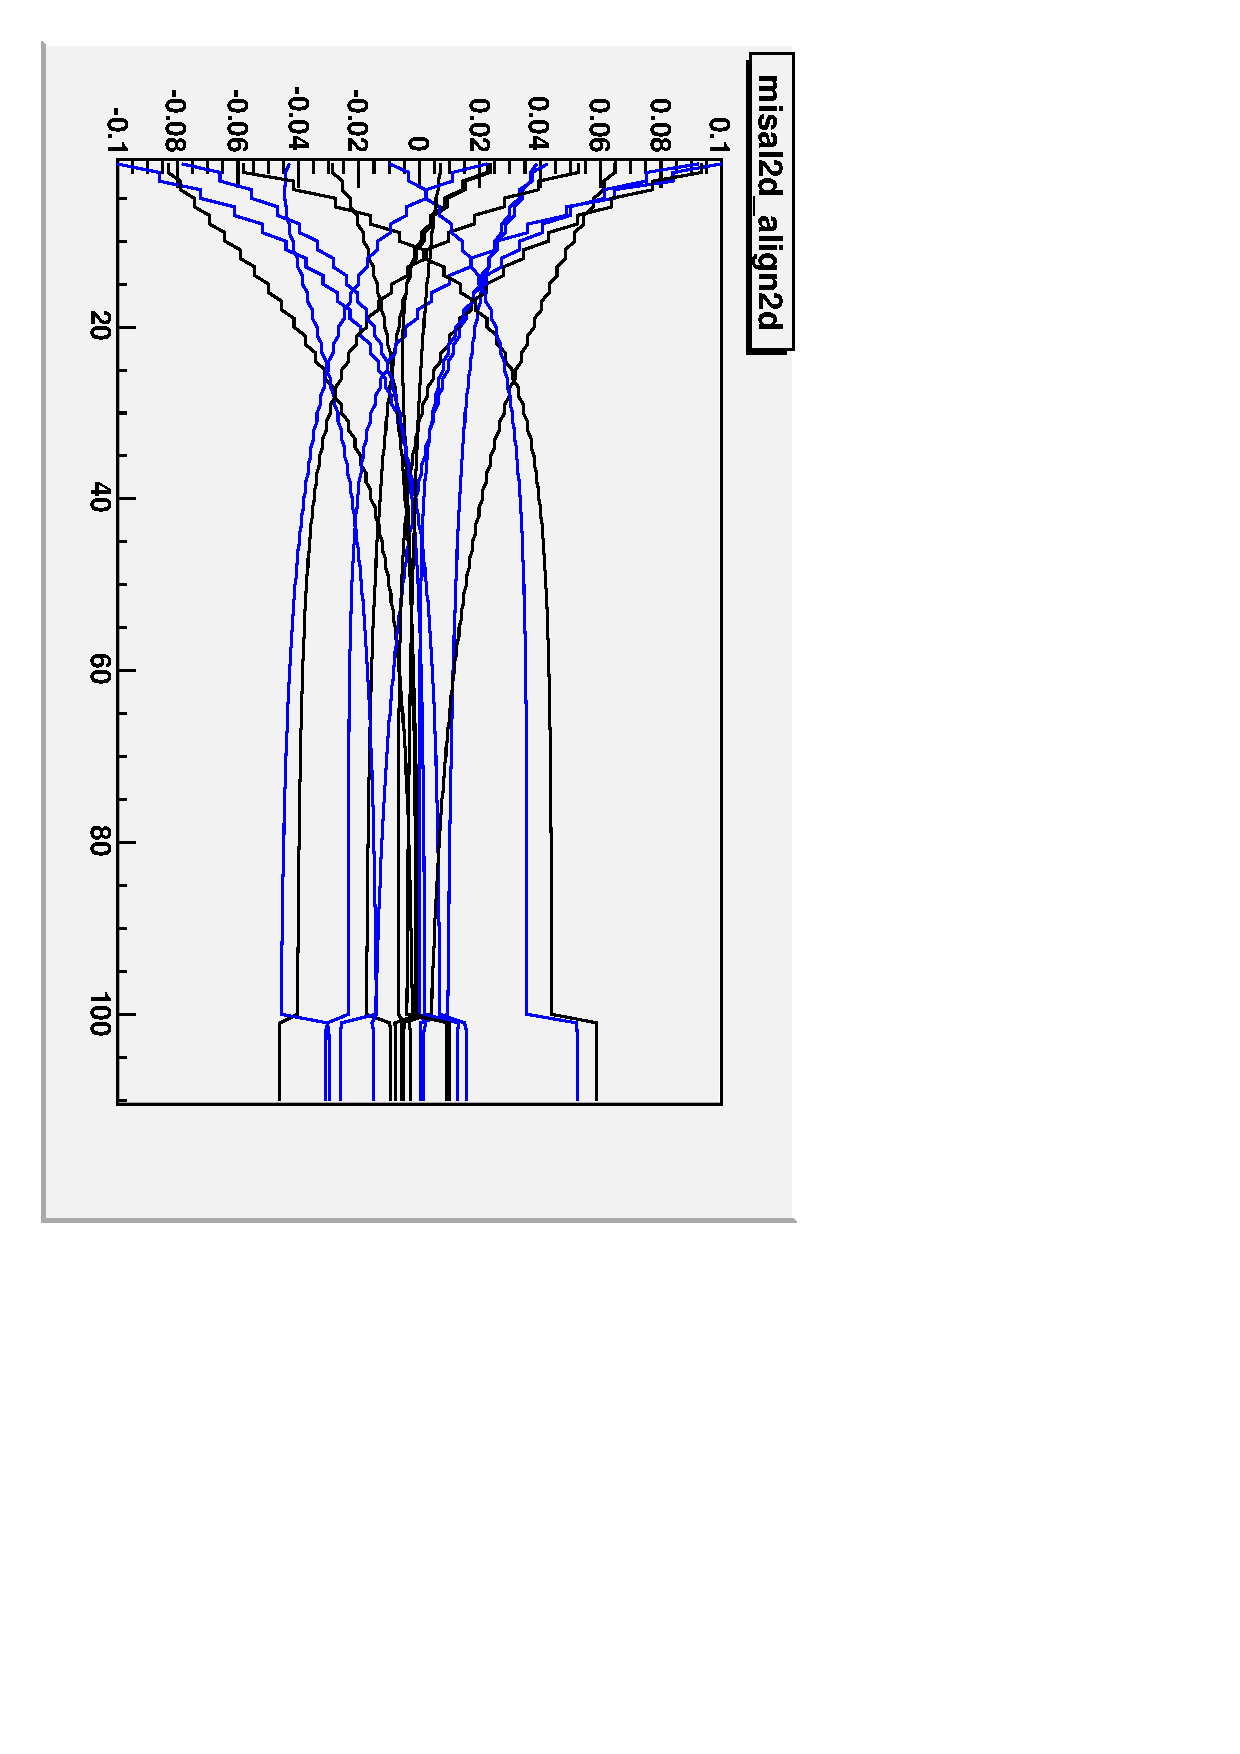
\includegraphics[height=0.9\linewidth, angle=90]{misal2d_align2d_lookx.pdf}}
\only<3>{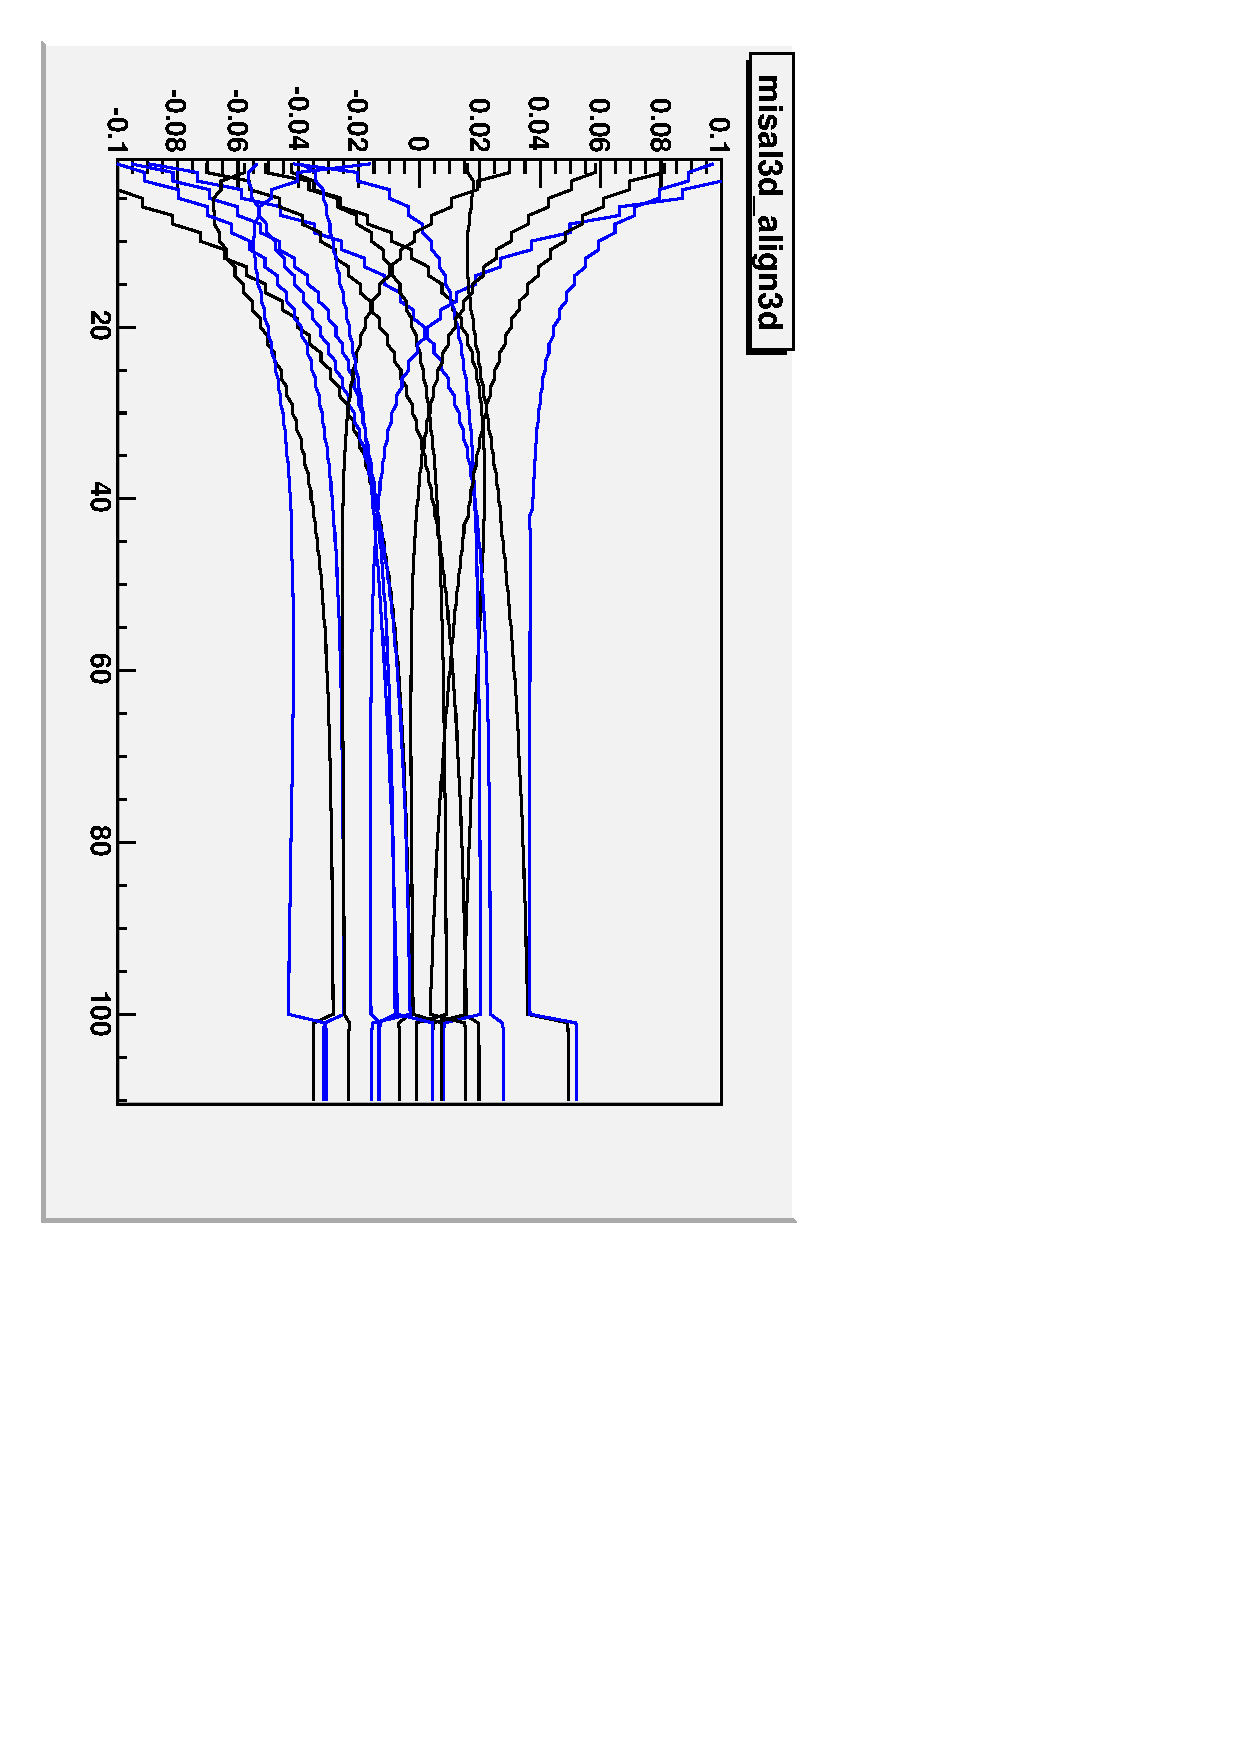
\includegraphics[height=0.9\linewidth, angle=90]{misal3d_align3d_lookx.pdf}}
\only<4>{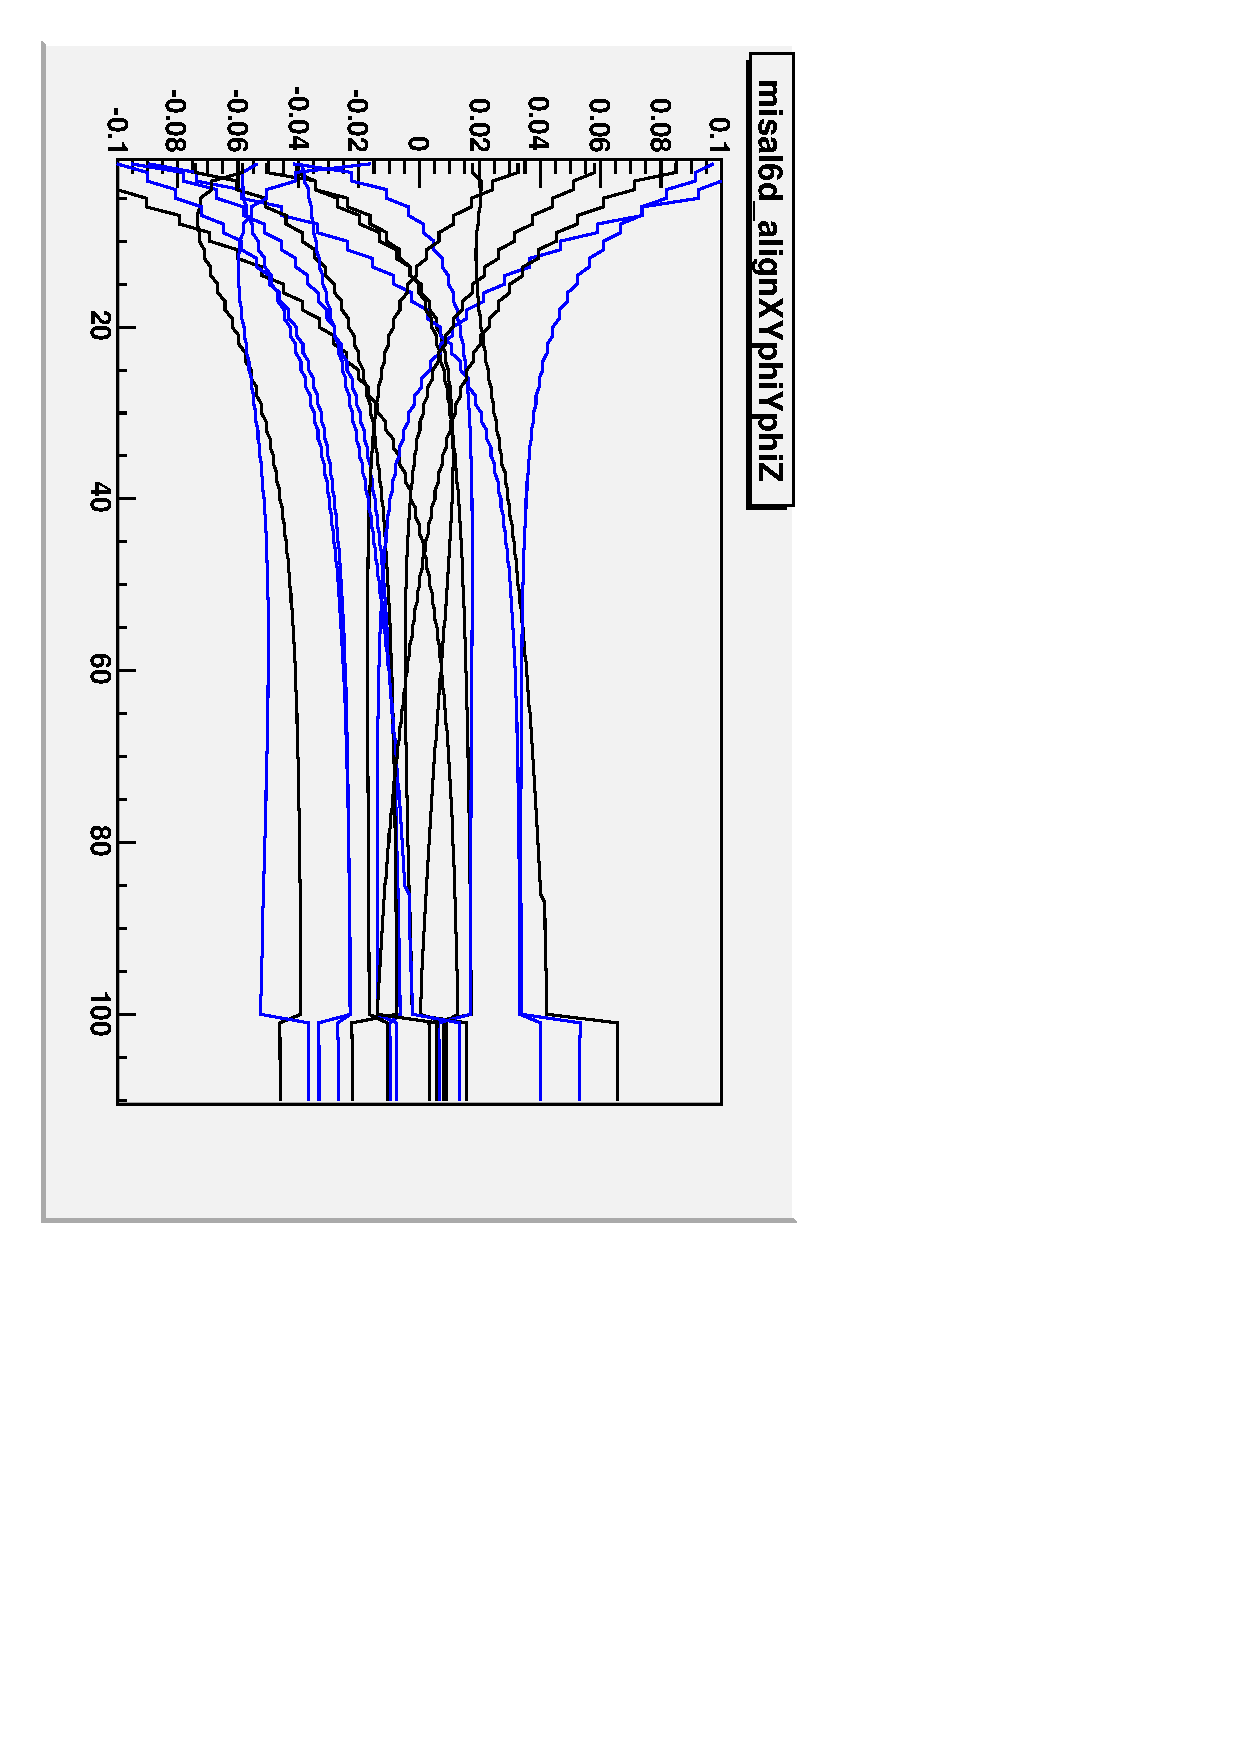
\includegraphics[height=0.9\linewidth, angle=90]{misal6d_alignXYphiYphiZ_lookx.pdf}}
\only<5>{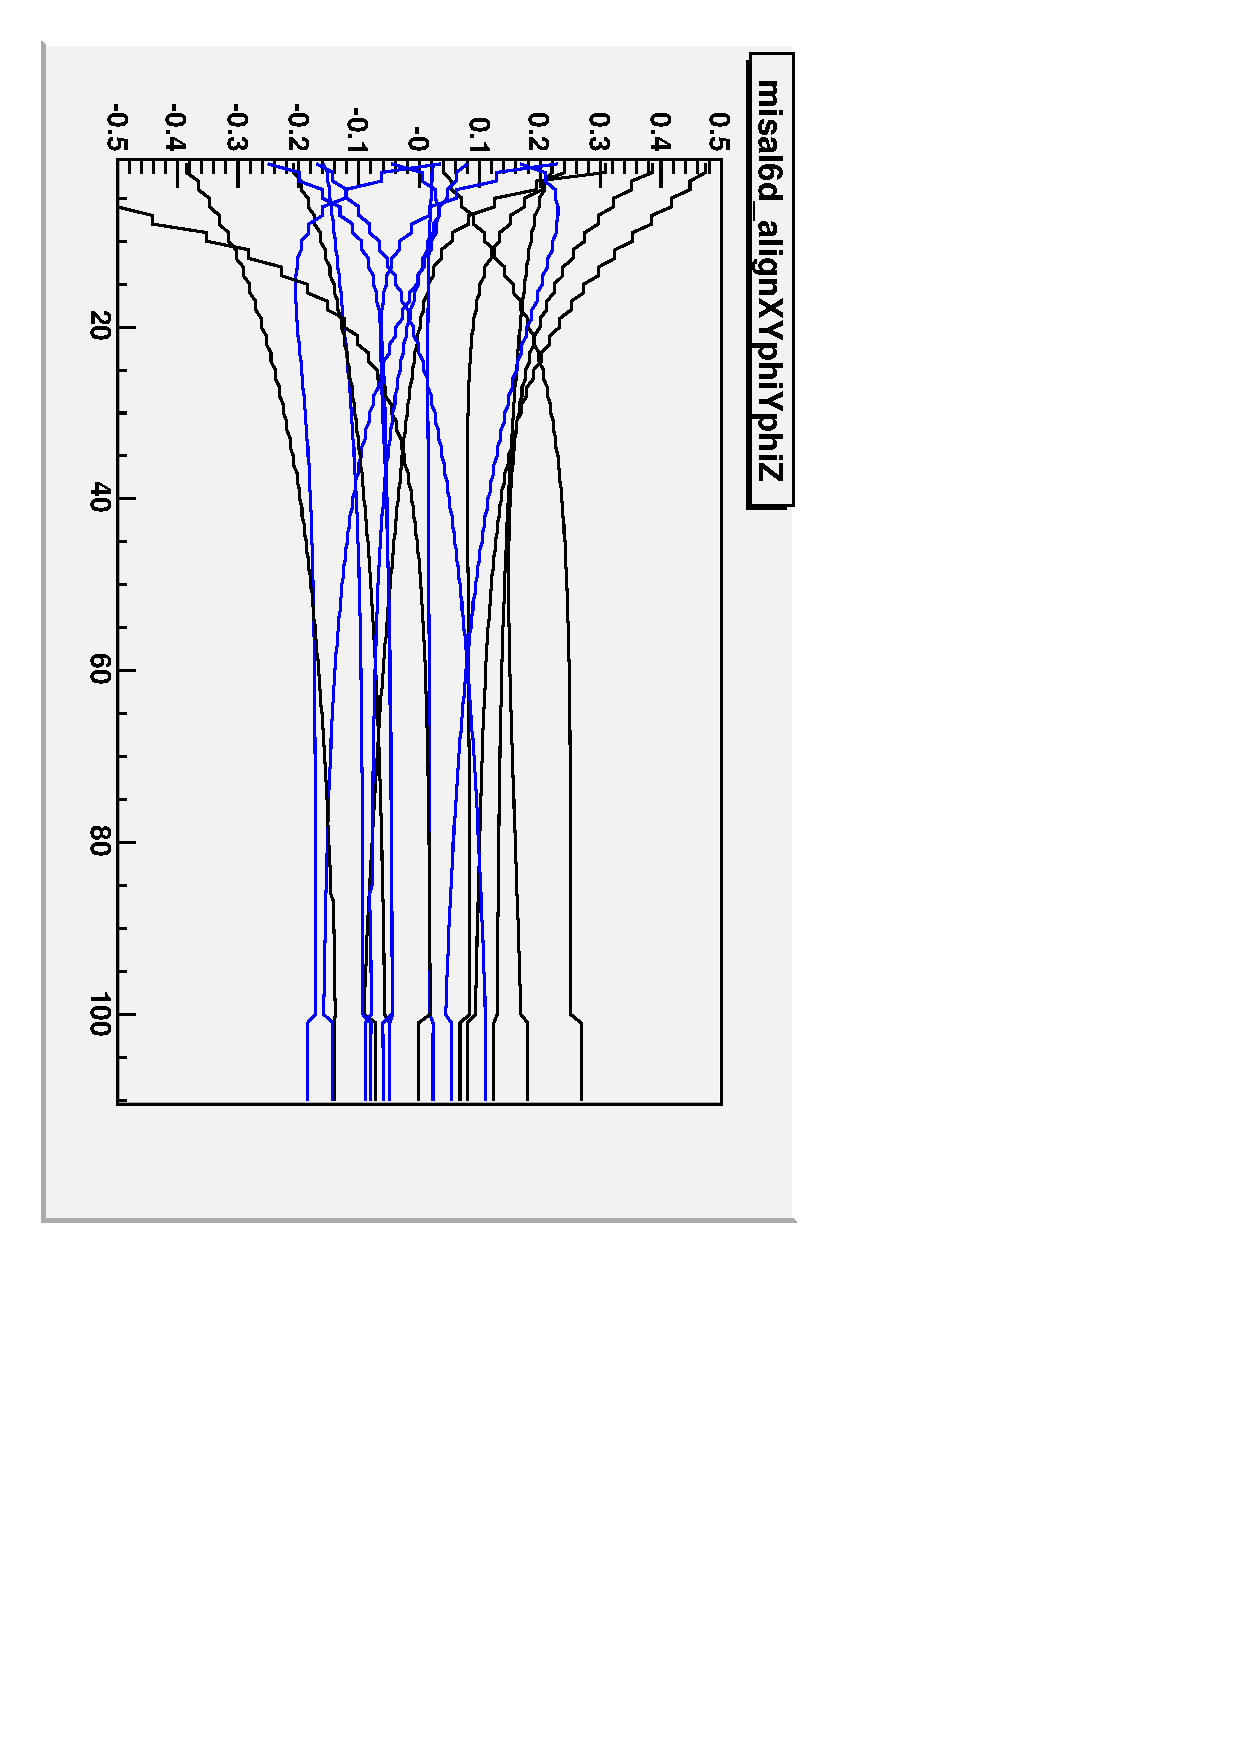
\includegraphics[height=0.9\linewidth, angle=90]{misal6d_alignXYphiYphiZ_looky.pdf}}
\only<6>{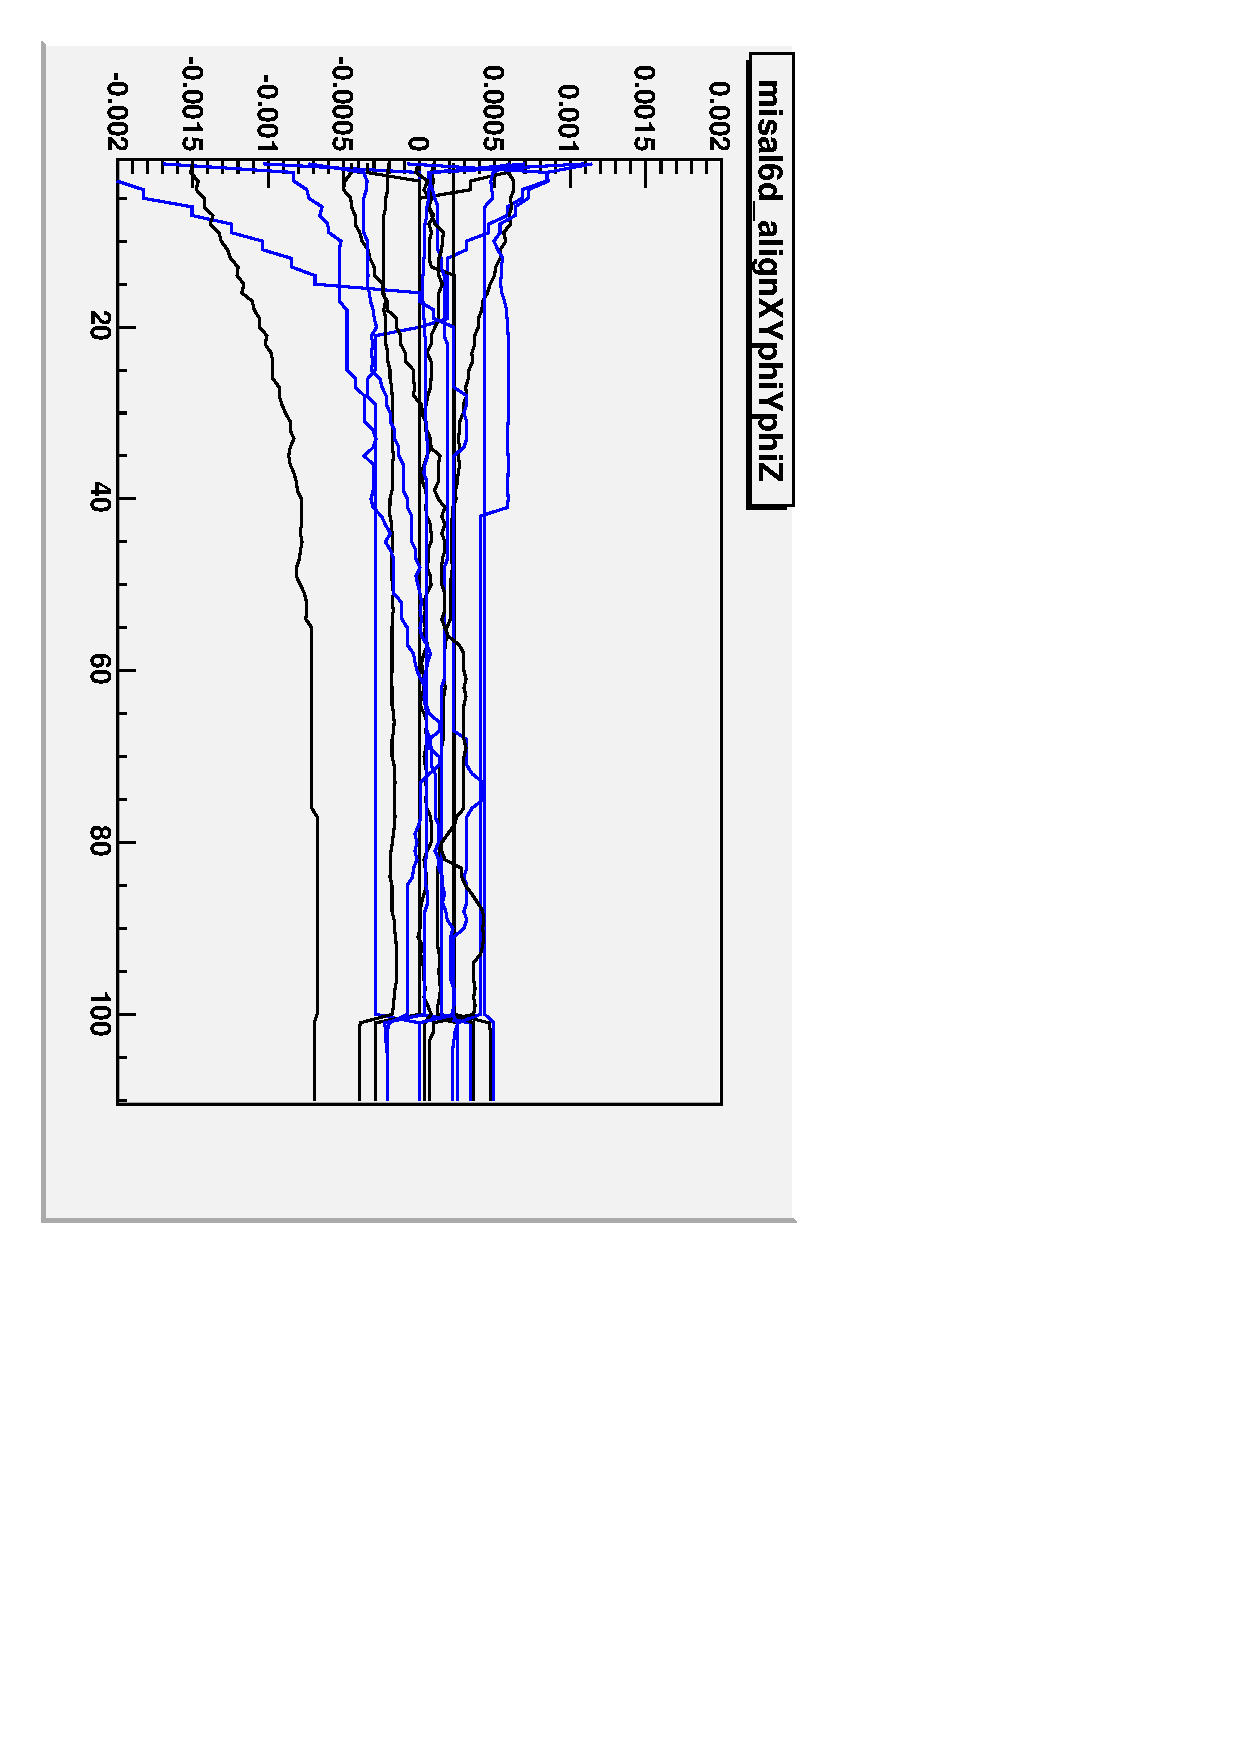
\includegraphics[height=0.9\linewidth, angle=90]{misal6d_alignXYphiYphiZ_lookphiy.pdf}}
\only<7>{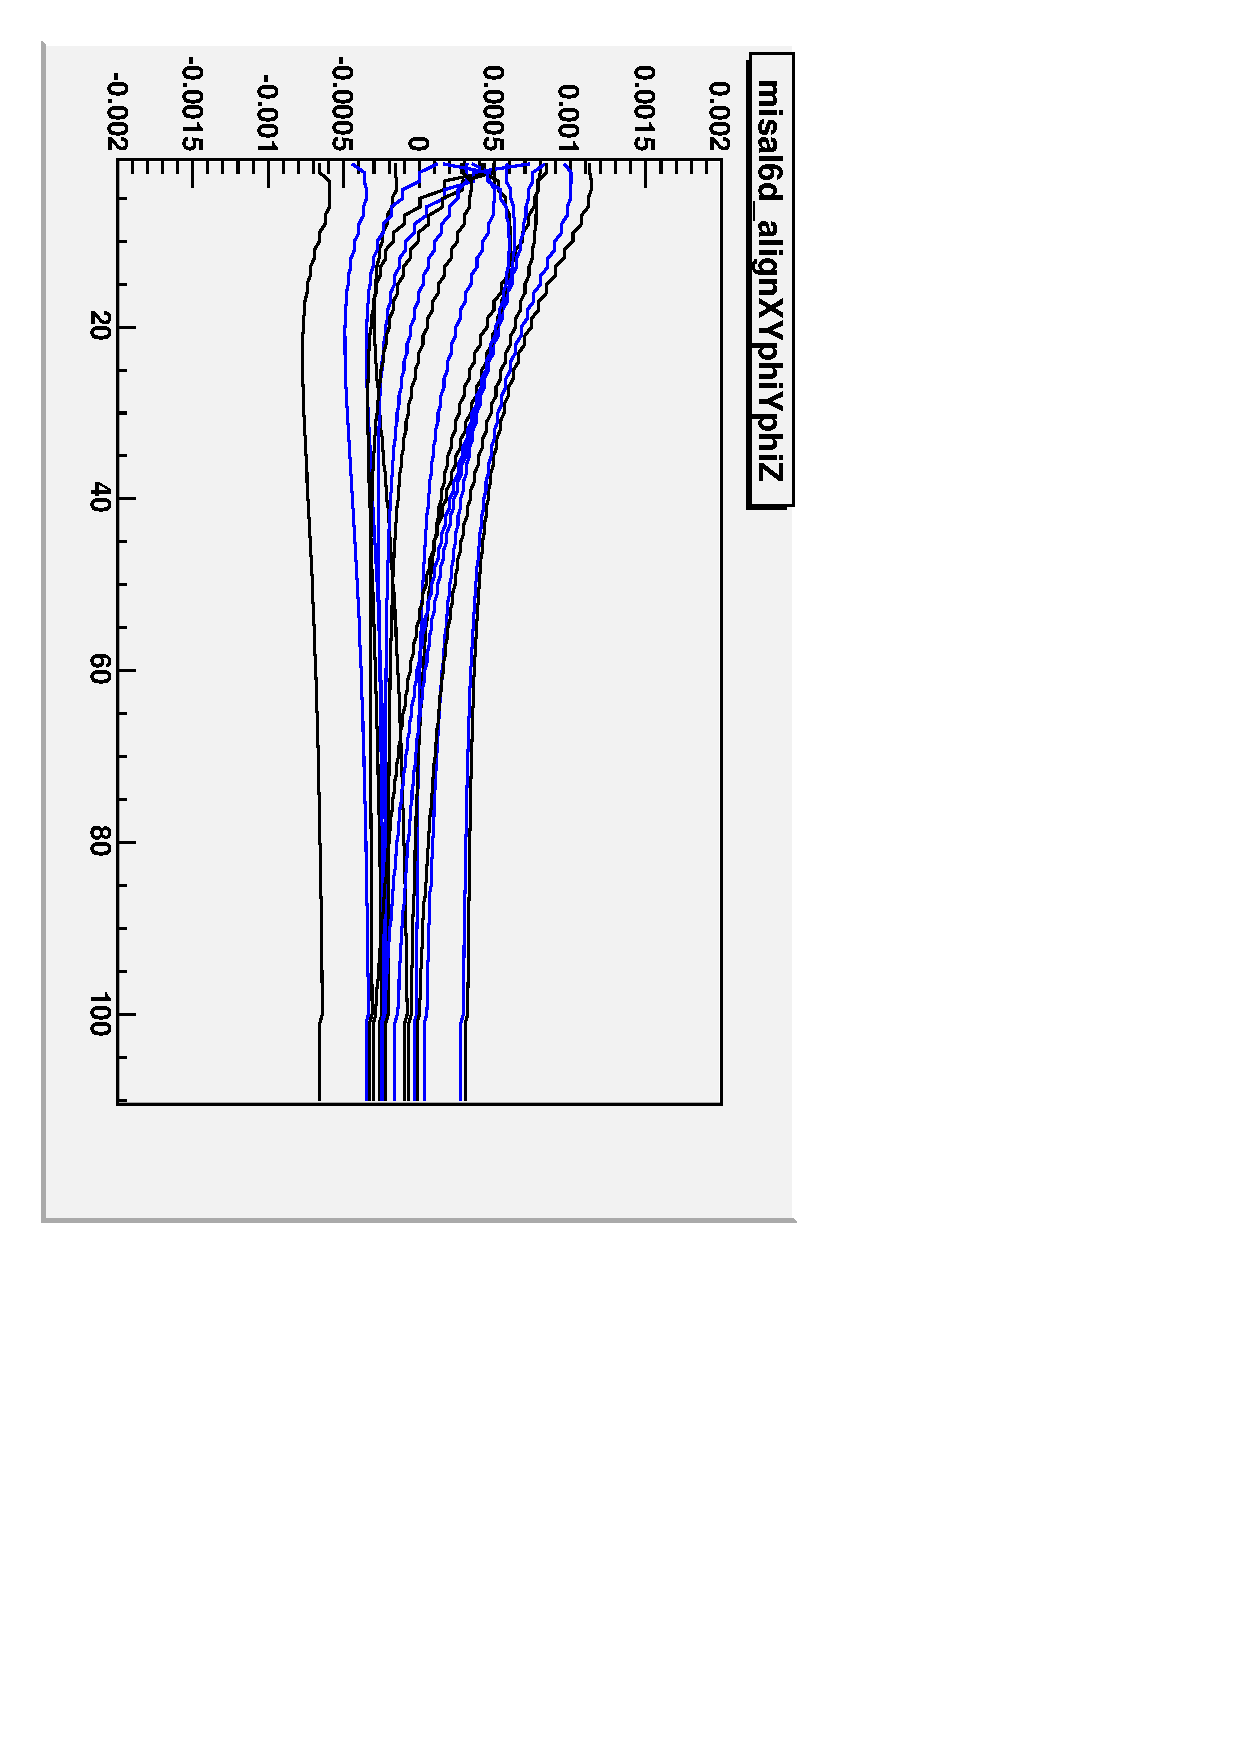
\includegraphics[height=0.9\linewidth, angle=90]{misal6d_alignXYphiYphiZ_lookphiz.pdf}}
\end{center}

\small Black are odd-numbered chambers, \textcolor{blue}{blue are
even,} \only<1-5>{cm}\only<6-7>{rad} from ideal position versus iteration, switch to global CSC
ring alignment at iteration 100.

\textcolor{red}{\only<1>{Only $x$ is misaligned.}\only<2>{$x$ and $y$ are misaligned.}\only<3>{$x$, $y$, and $\phi_z$ are misaligned.}\only<4-7>{All DOF are misaligned; $x$, $y$, $\phi_y$, and $\phi_z$ are re-aligned.}}

\end{frame}

\begin{frame}
\frametitle{Baseline procedure: \only<1>{new barrel}\only<2>{new endcap}\only<3-4>{old}}

\begin{center}
\only<1>{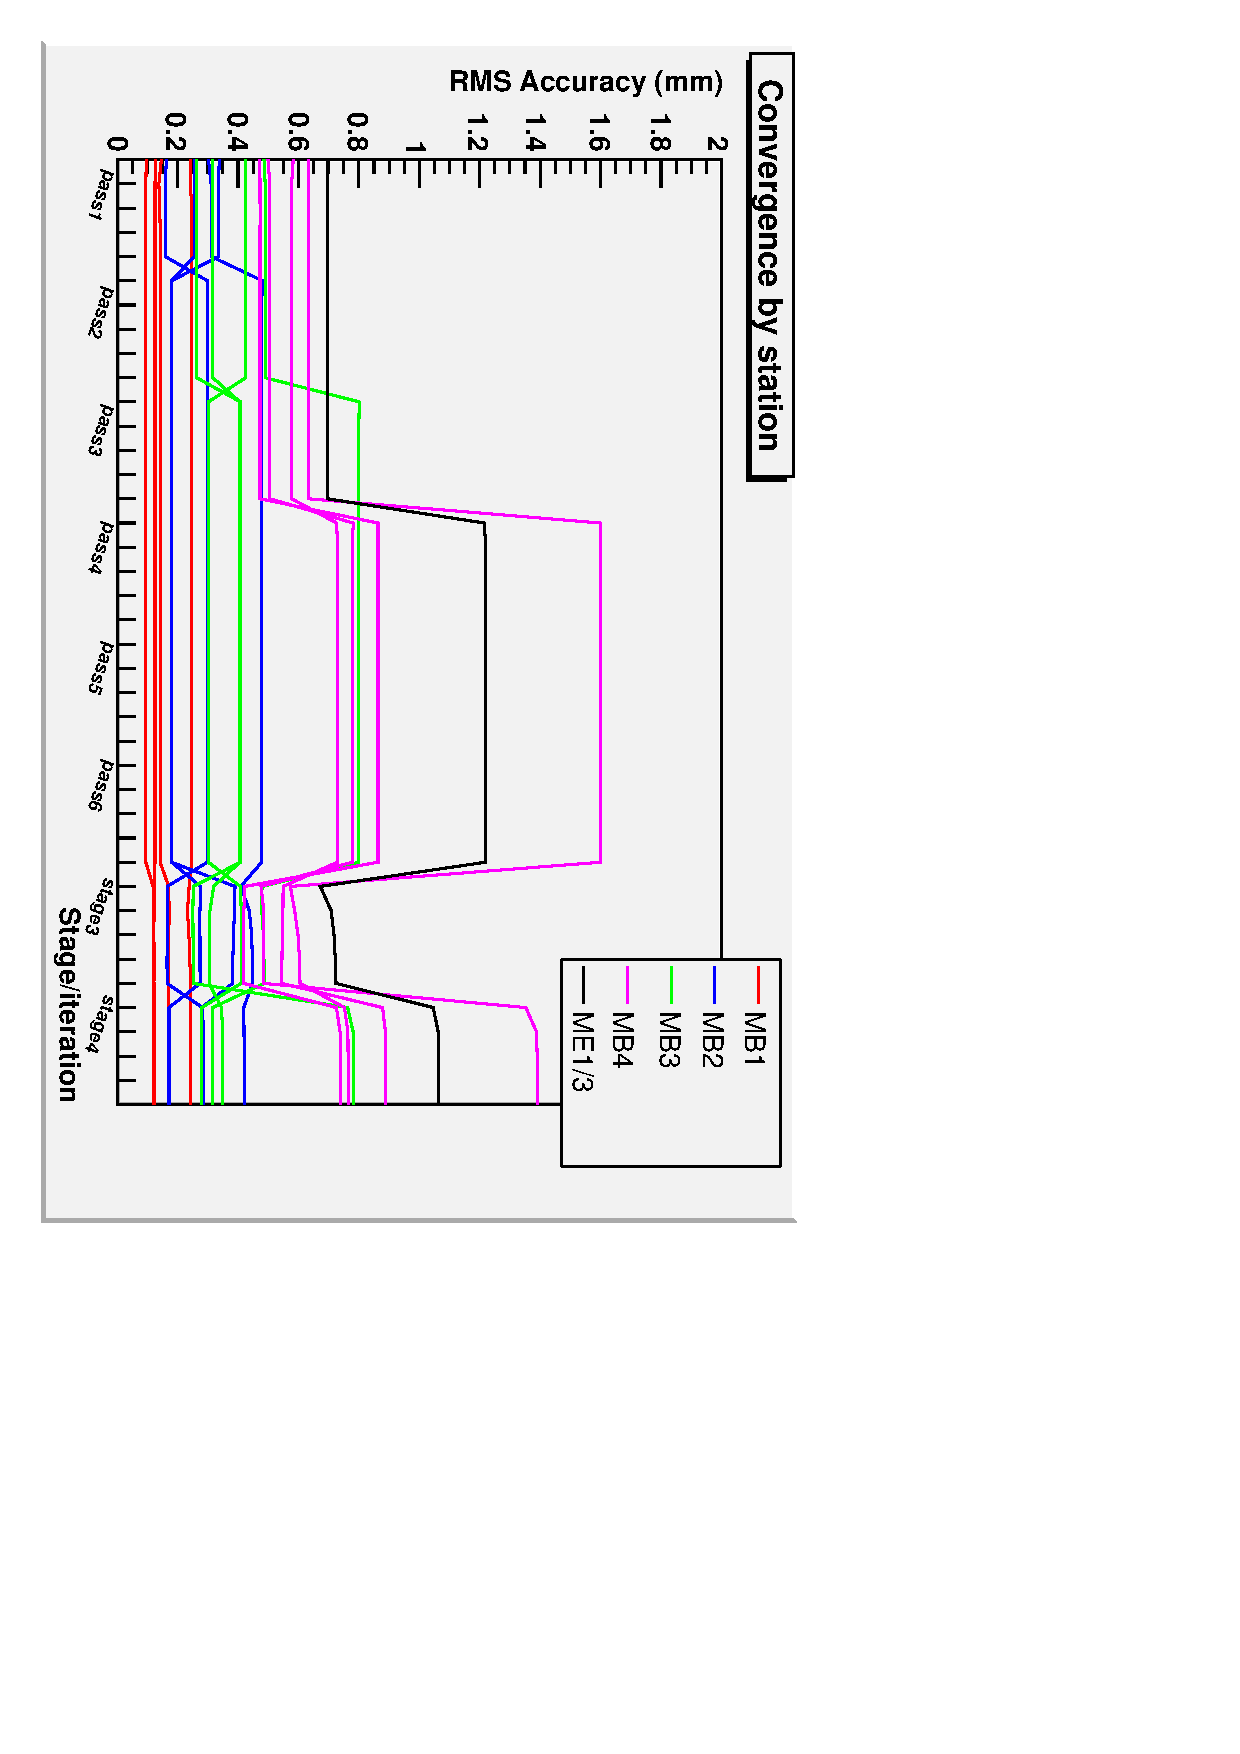
\includegraphics[height=0.9\linewidth, angle=90]{convergence_barrel.pdf}}
\only<2>{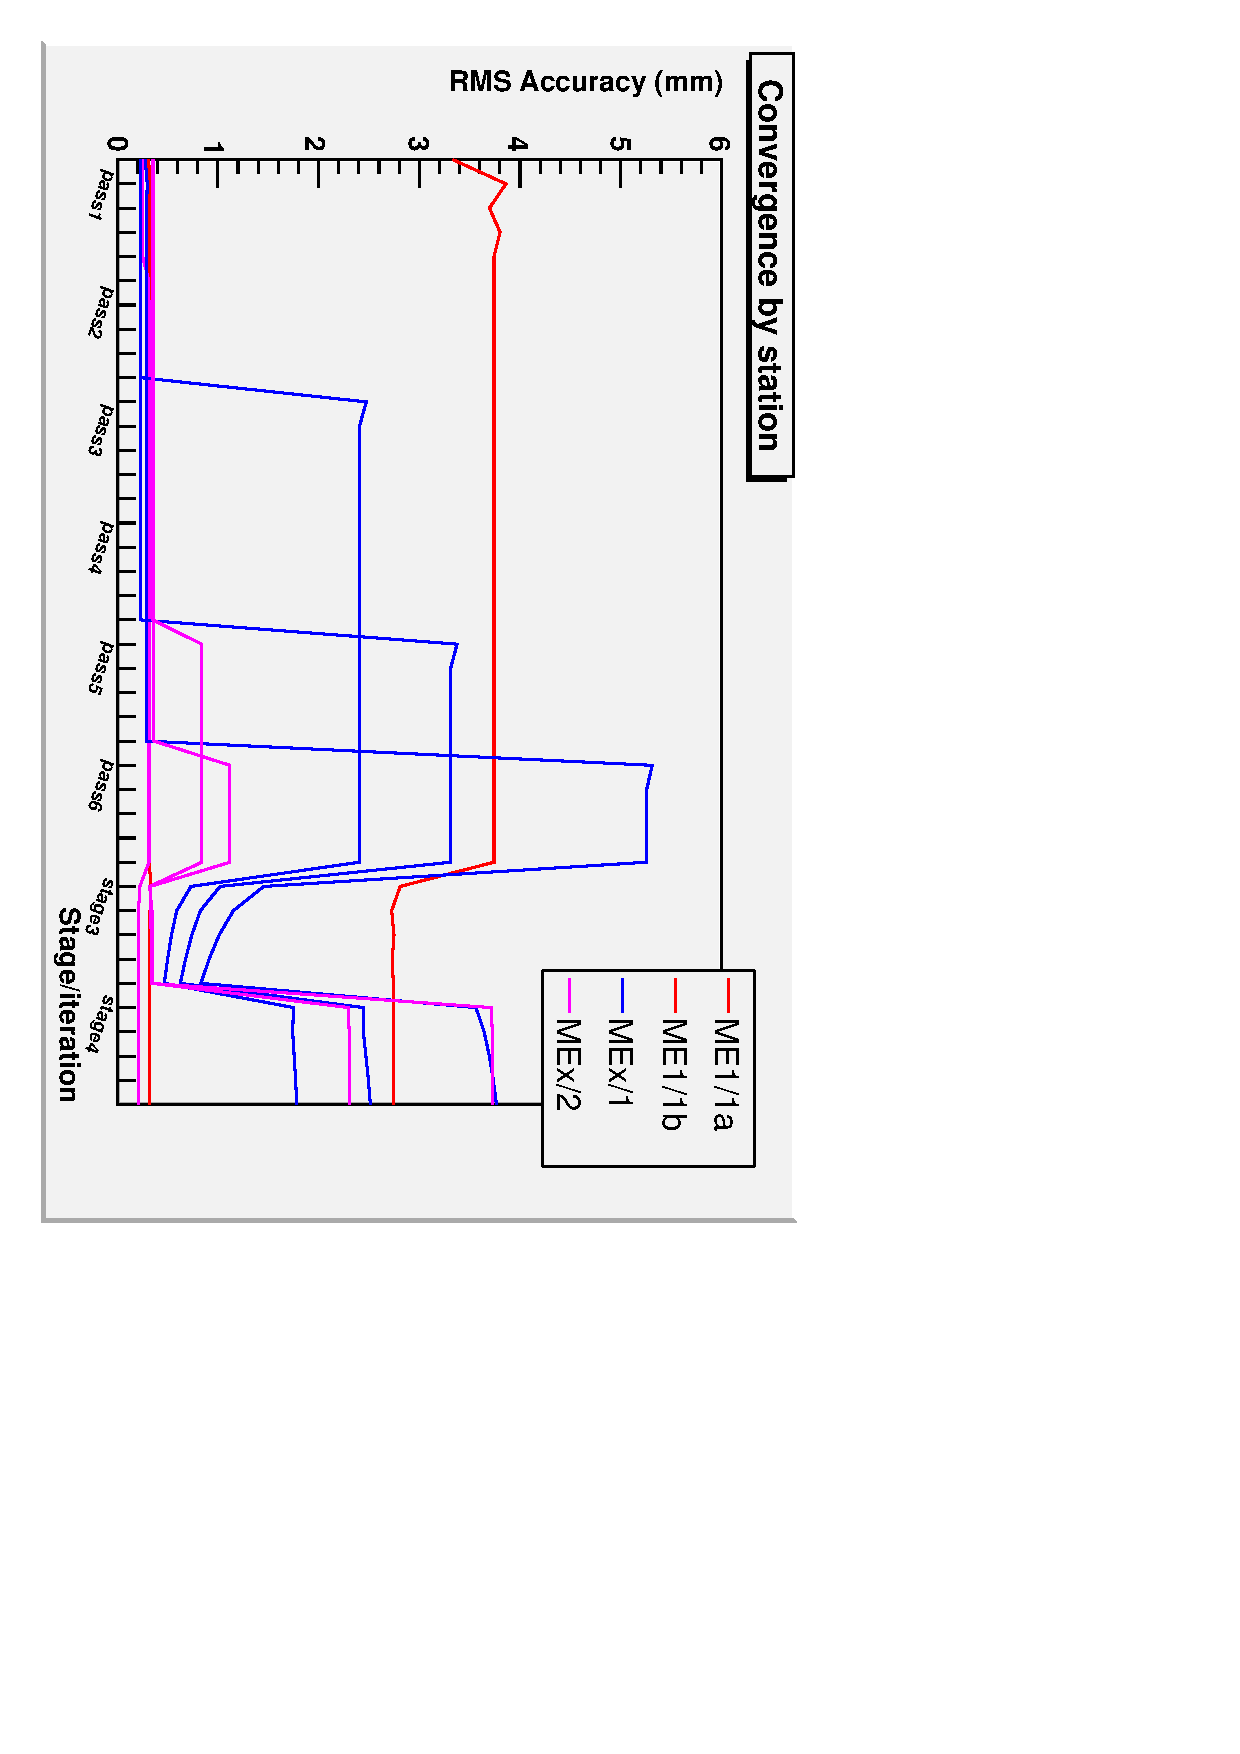
\includegraphics[height=0.9\linewidth, angle=90]{convergence_endcap.pdf}}
\only<3>{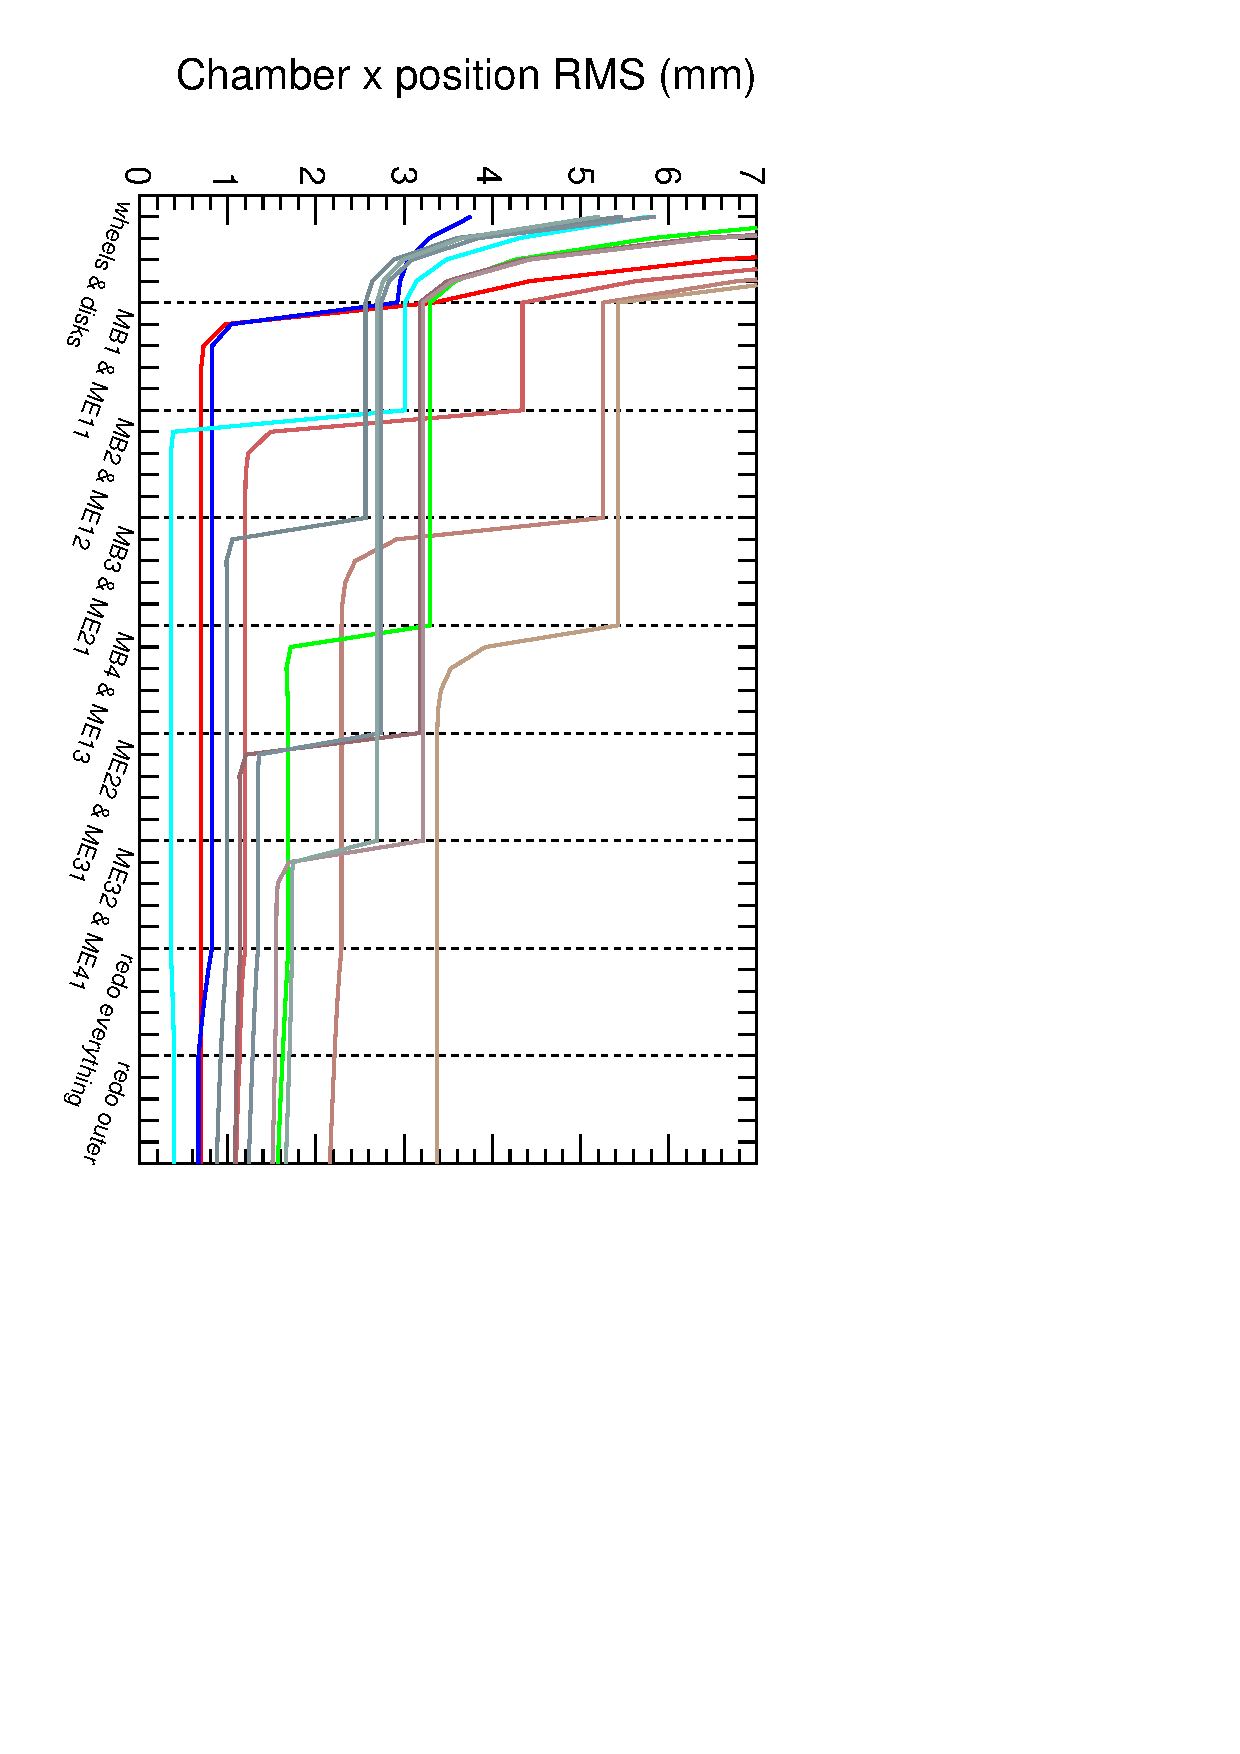
\includegraphics[height=0.9\linewidth, angle=90]{oldprocedure.pdf}}
\only<4>{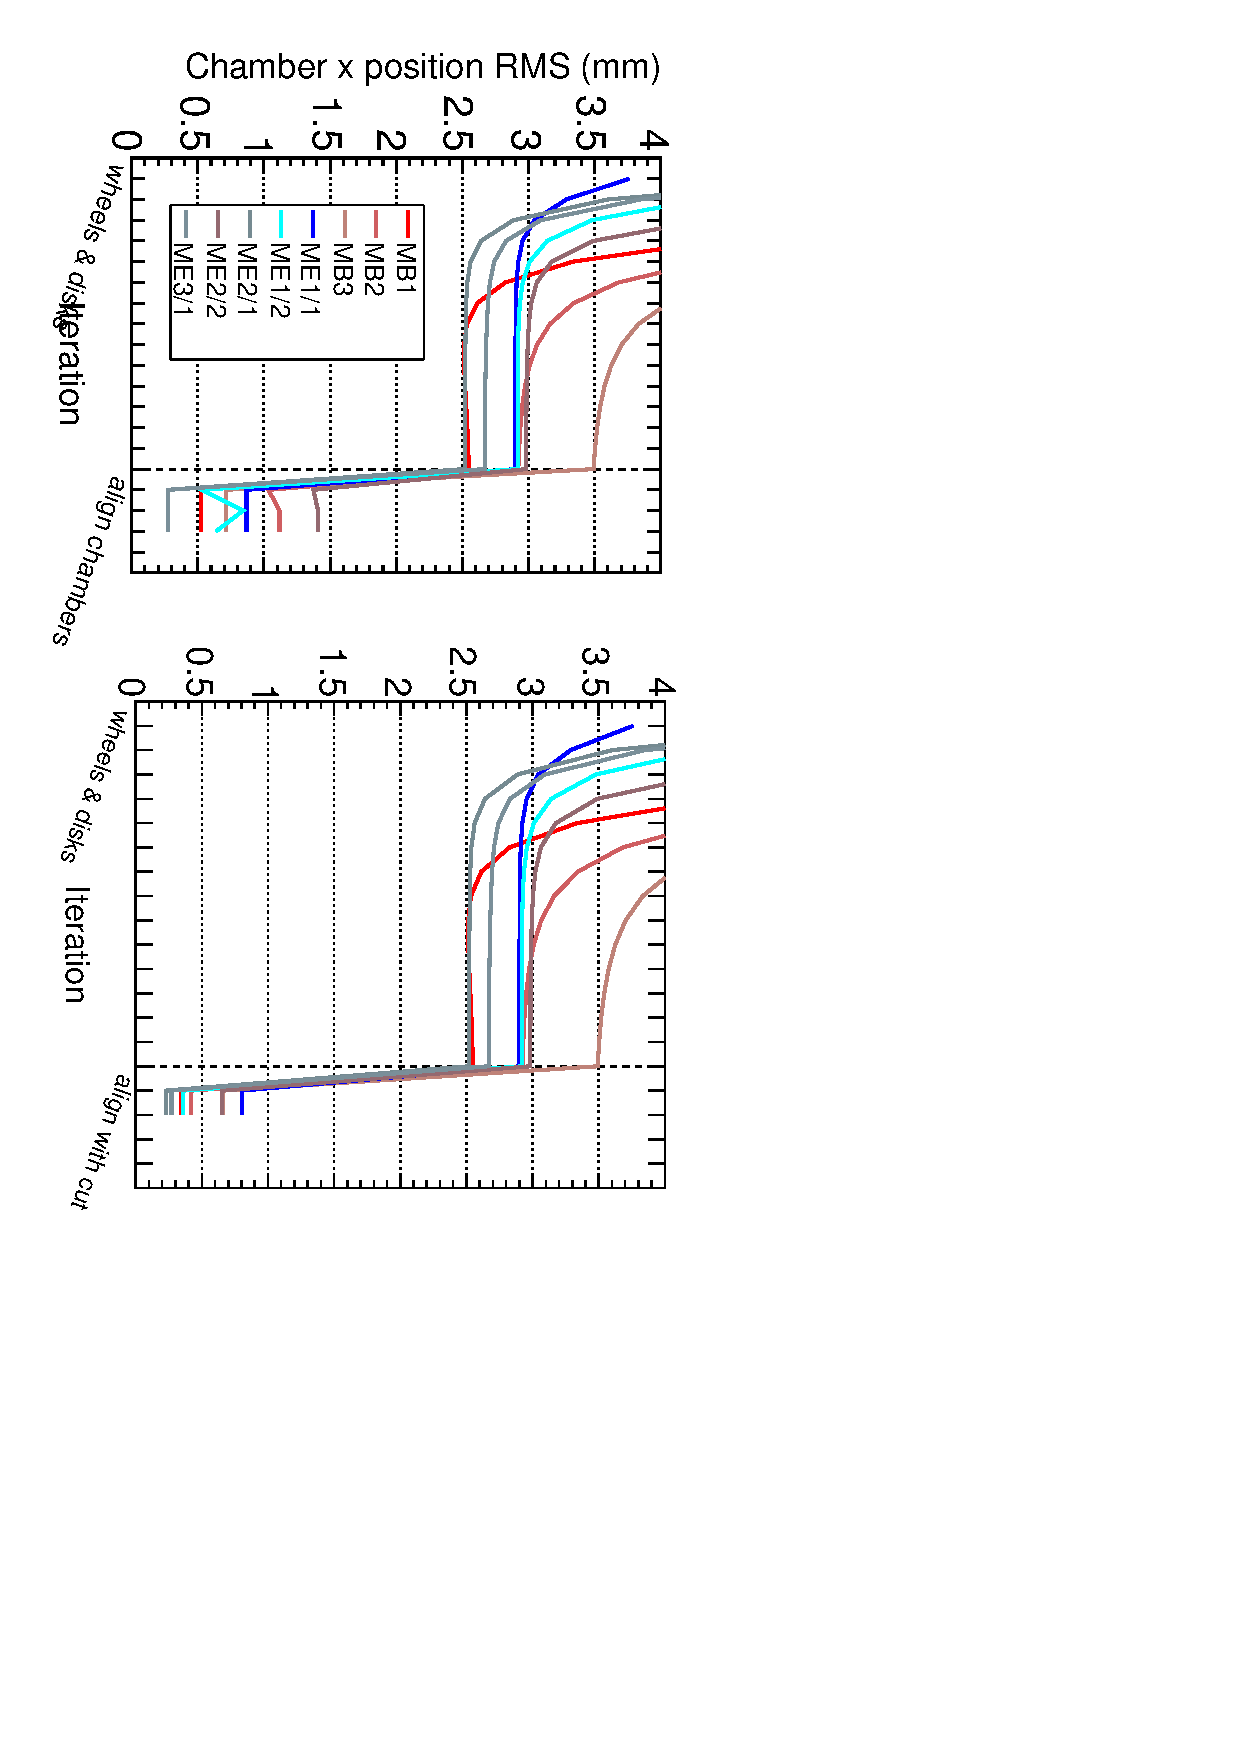
\includegraphics[height=0.9\linewidth, angle=90]{compate_with_without_cut.pdf}}
\end{center}

\small \only<1-2>{What we're looking at is {\it after} the wheel/disk
and first iteration.  Unlike old baseline, I allow {\it all} stations
to align with APE = $\infty$ in the first step.} \only<3>{Old baseline
had too few wheel/disk iterations using too much data.

Why don't I see improvement in stage 3 (redo everything)?  The stopping condition?}
\only<4>{Fairest comparison from old plots: one iteration {\it
without} track cut (left) after wheel/disk.  Old results are about
2$\times$ worse.}
\only<1>{Also, new APEs are only 0 and $\infty$, not carefully tuned.}
\only<2>{The outlying ME1/1b is clearly a bug.}
\end{frame}

\begin{frame}
\frametitle{Luminosity scaling: \only<1>{barrel}\only<2>{endcap}}
\only<1>{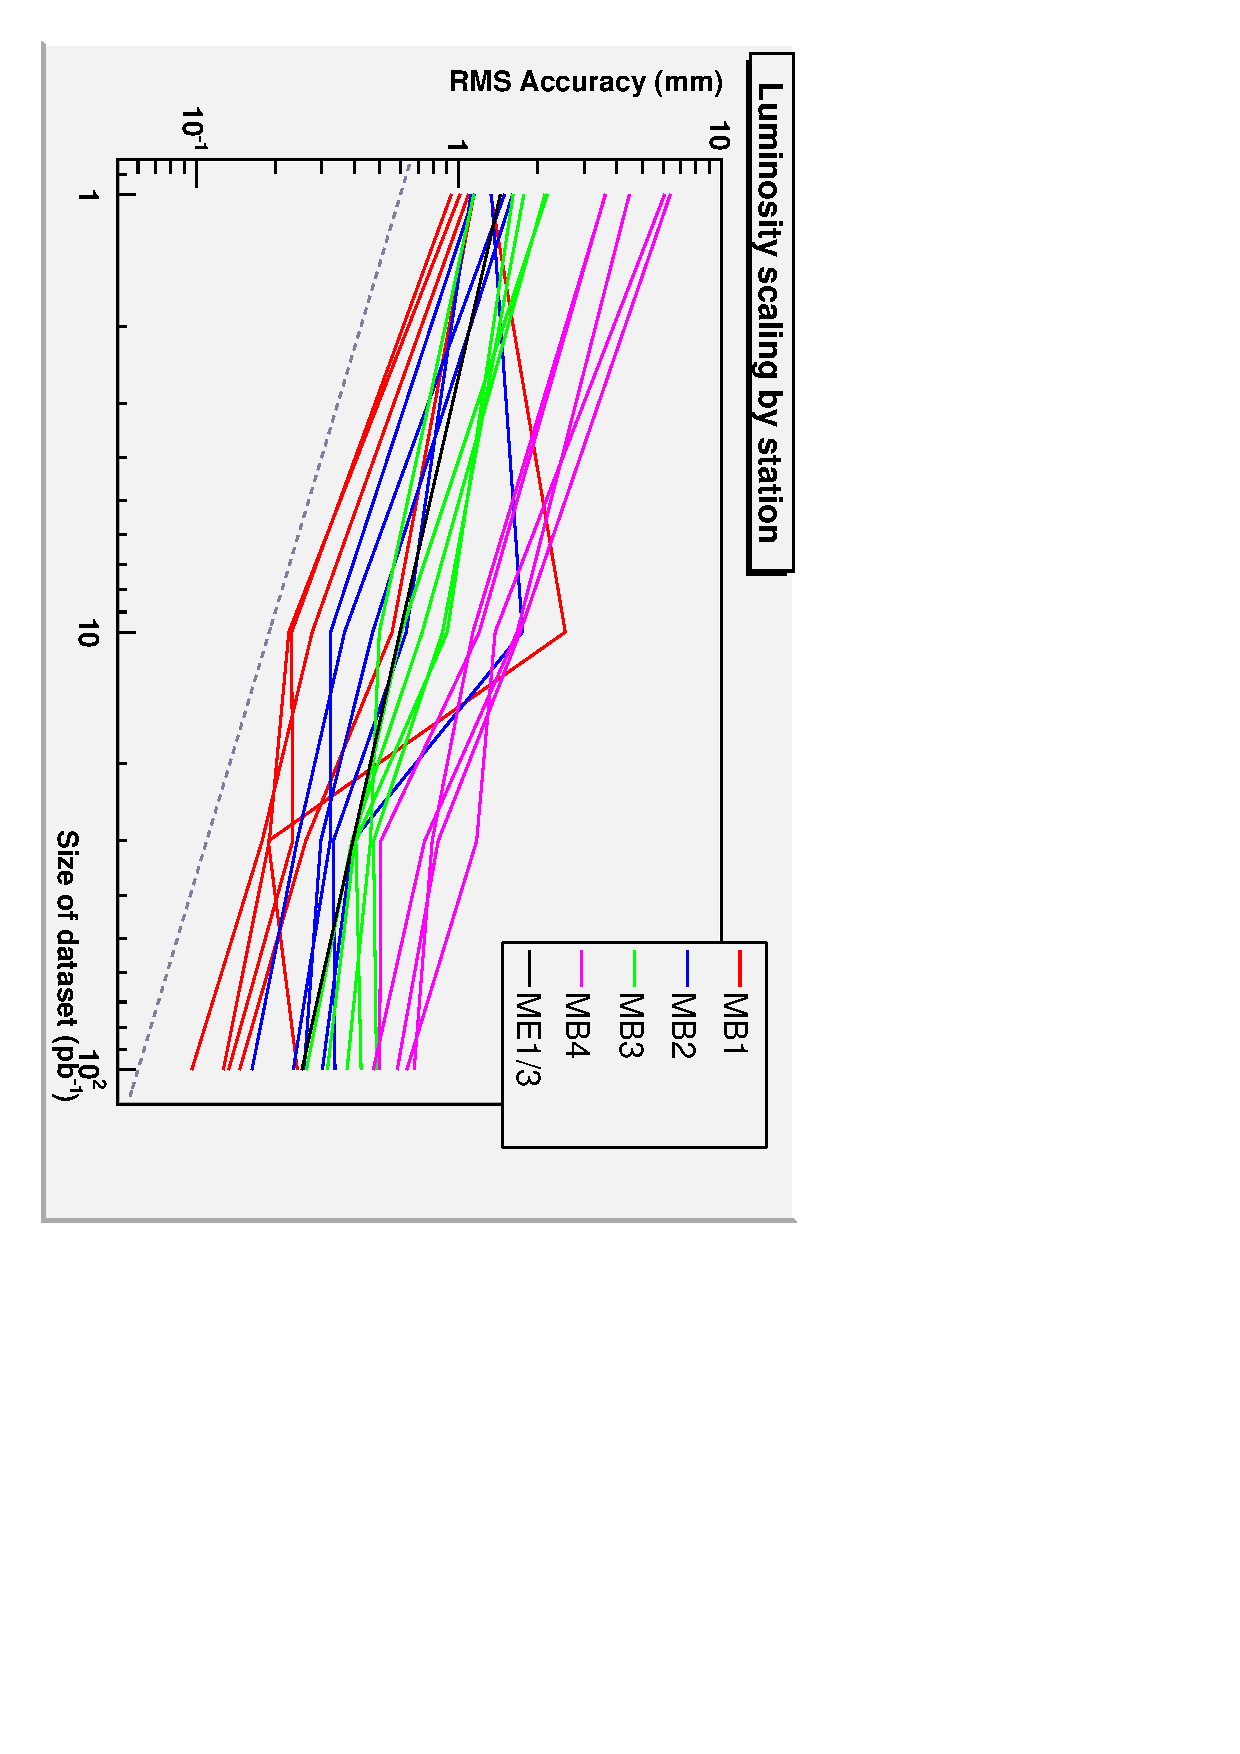
\includegraphics[height=\linewidth, angle=90]{scaling_barrel.pdf}}
\only<2>{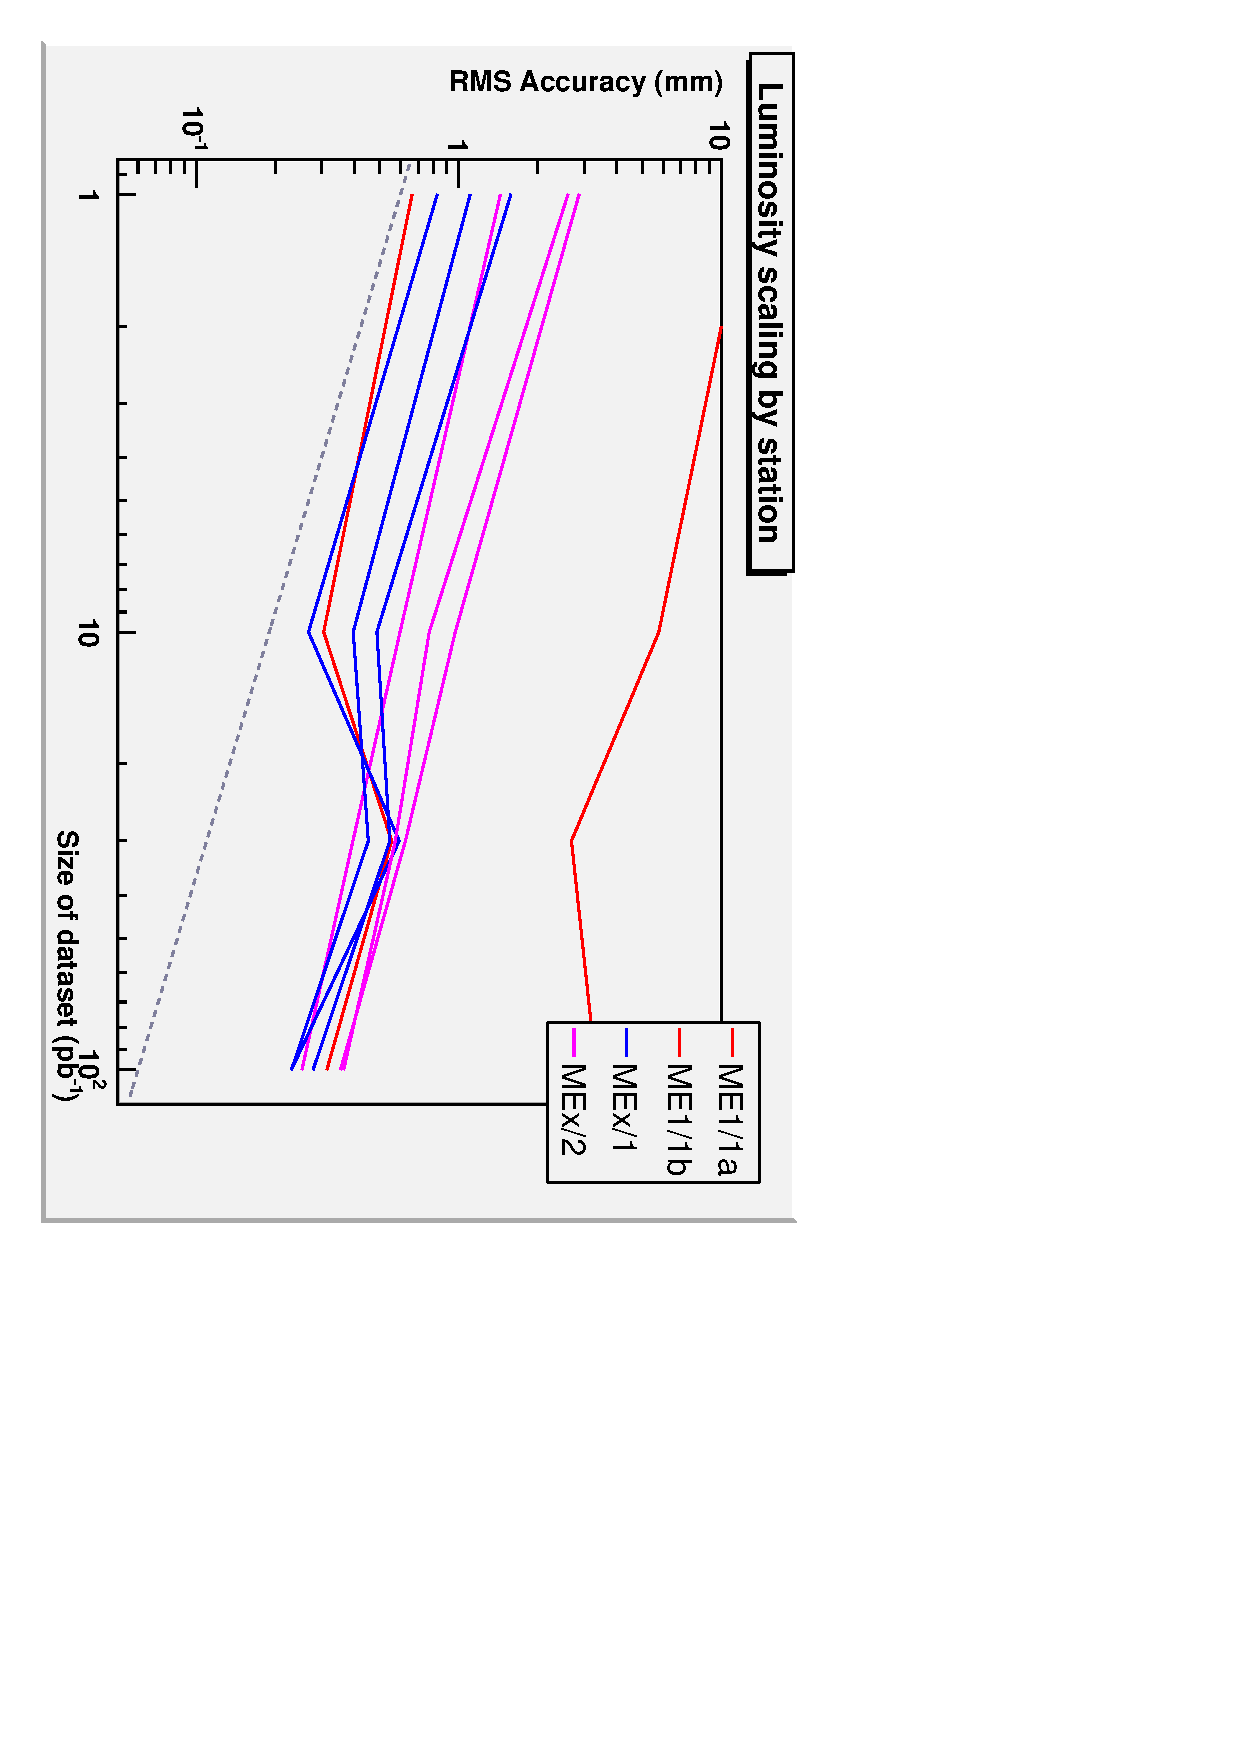
\includegraphics[height=\linewidth, angle=90]{scaling_endcap.pdf}}

\small (using the new procedure)

\only<1>{Kinks at 10~$pb^{-1}$ are due to single chambers in
\textcolor{red}{ME2/1} and \textcolor{blue}{ME2/2}.}
\end{frame}

\begin{frame}
\frametitle{Worst chambers: \only<1>{barrel}\only<2>{endcap}}
\only<1>{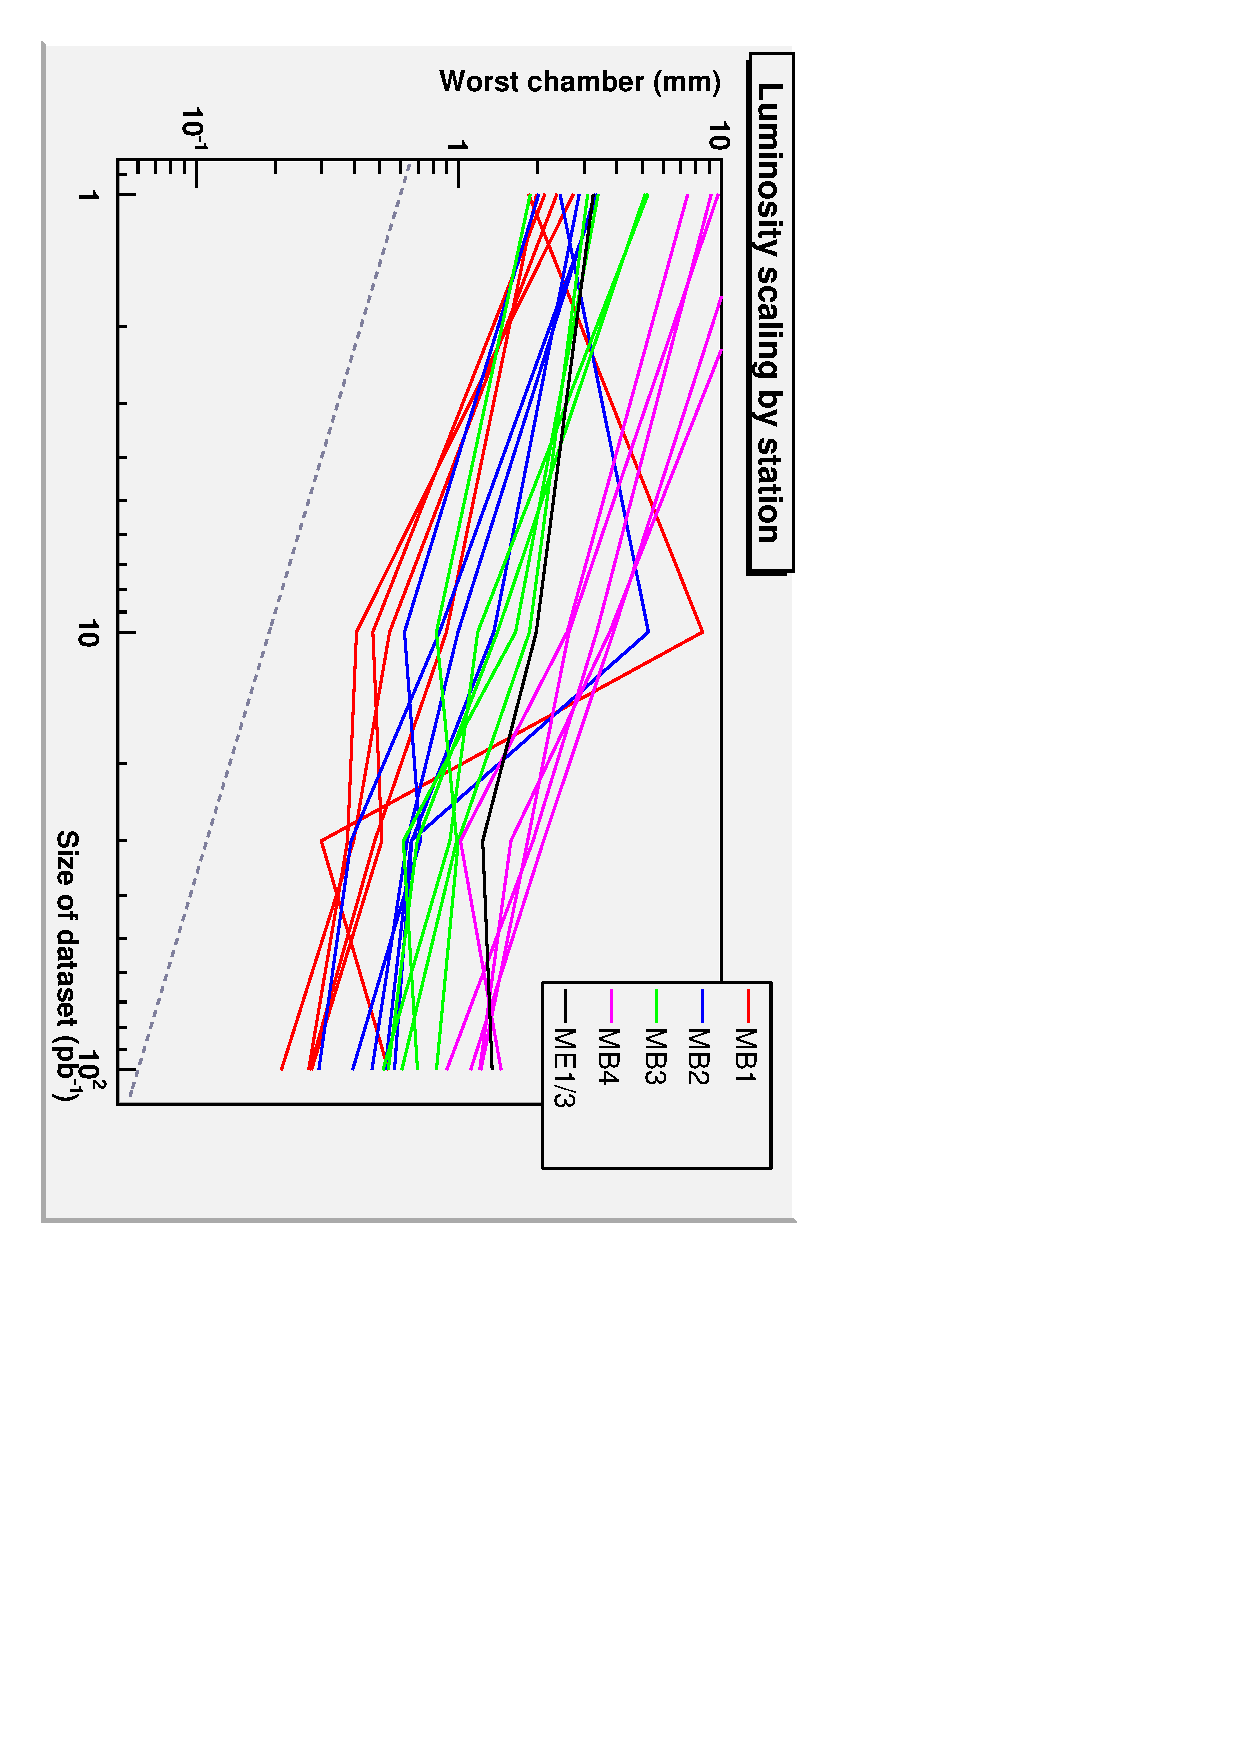
\includegraphics[height=\linewidth, angle=90]{worst_barrel.pdf}}
\only<2>{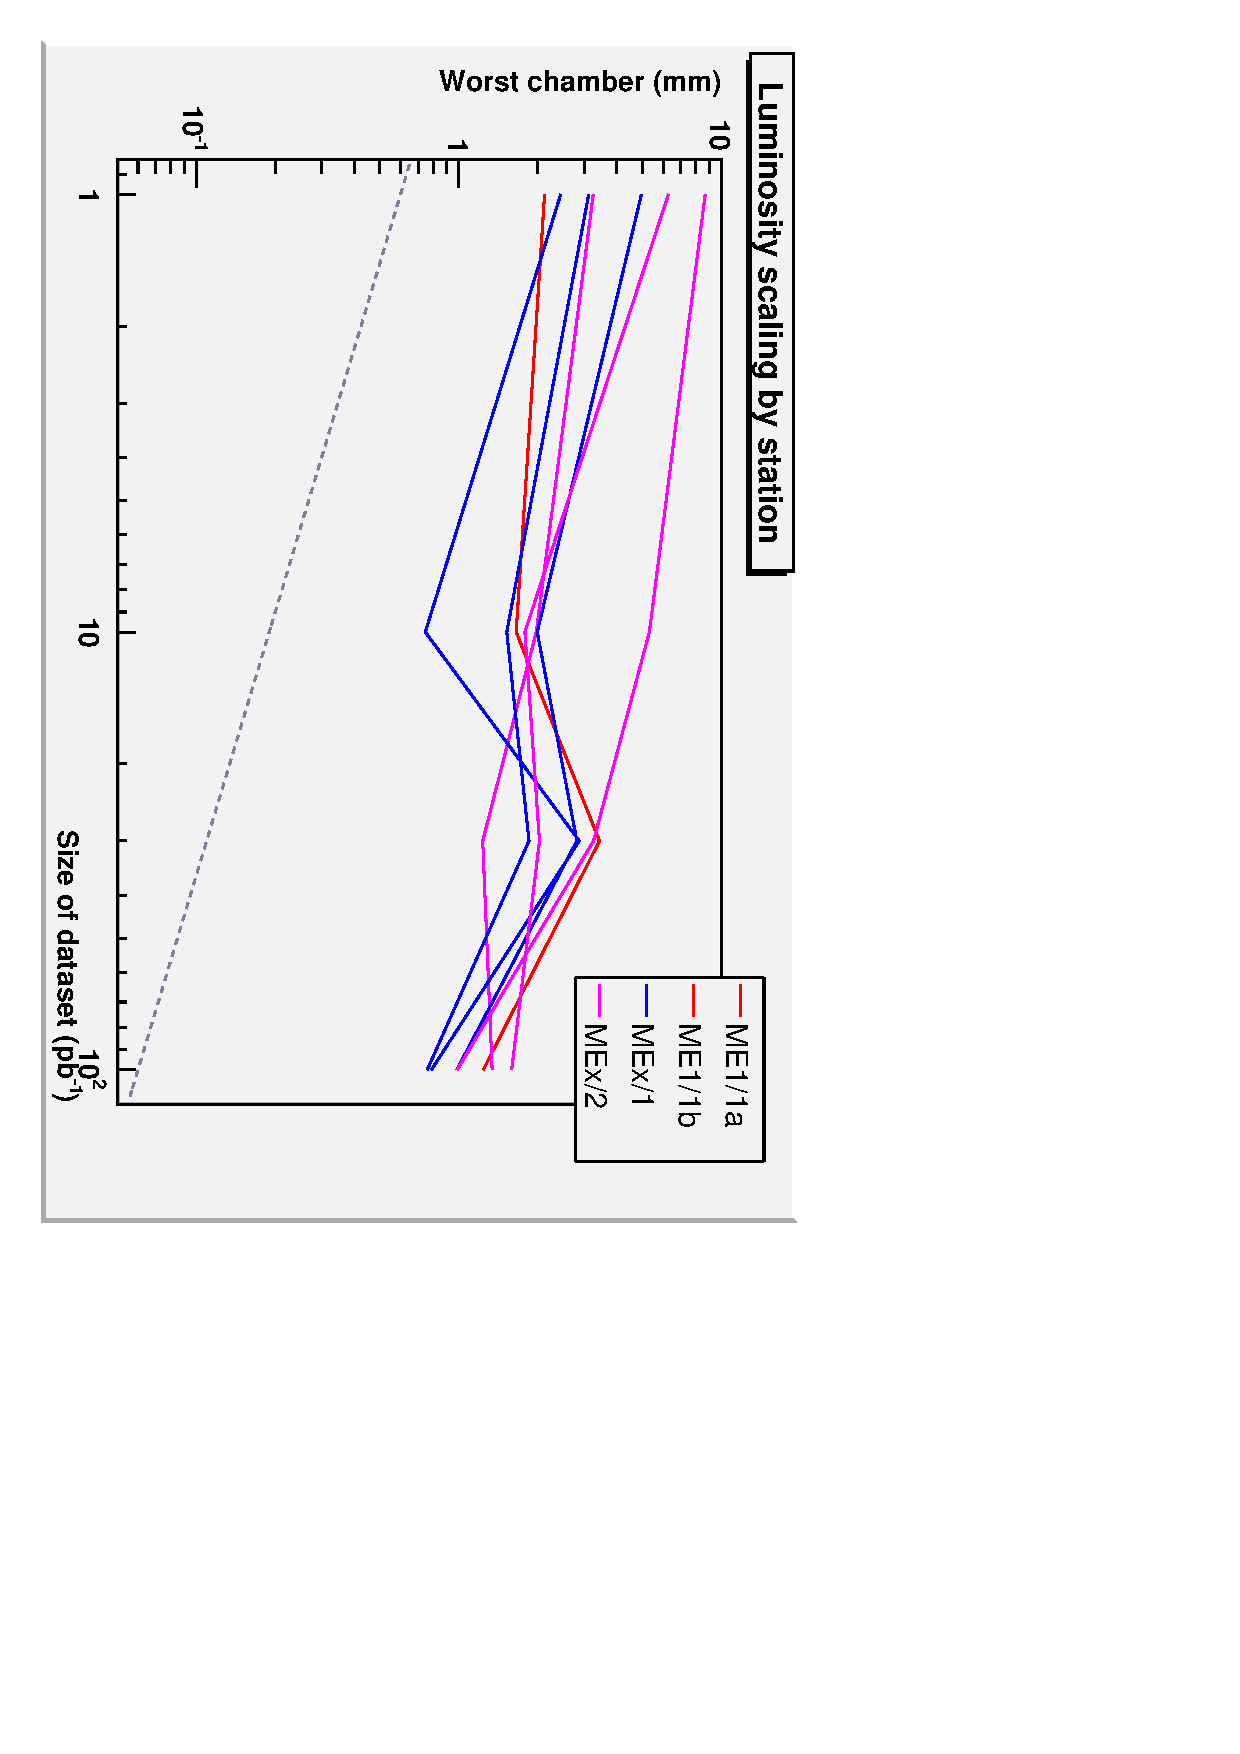
\includegraphics[height=\linewidth, angle=90]{worst_endcap.pdf}}

\small (using the new procedure)
\end{frame}

\begin{frame}
\frametitle{Survey constraints}

\small
By actually attempting to do an alignment with survey constraints, I found some show-stoppers and near-show-stoppers:
\begin{itemize}
\item The constraint has only been implemented with 6 degrees of
freedom.  MB4 cannot and CSCs should not be allowed to align in all 6
degrees of freedom.  Someone would need to make the implementation
more general to use it in the muon system.
\item We wanted to use the constraints to rein in chambers that wander
due to wierd tracks (multiple scattering).  That suggests that the
weight of the constraint should scale with the number of hits, so that
we can set the degree of competition between hits and constraints
independently of the number of hits on a chamber.  They actually
designed a constraint that does not depend on the number of hits; it
seems to be intended to fill in for missing track data.
\item The software assumes that we would never align objects that are
not direct descendents of each other in the hierarchy: DTChambers and
CSCChambers are third cousins.  That's surmountable, but may require
some interface changes.
\end{itemize}

\end{frame}


%% \begin{frame}
%% \frametitle{Outline}
%% \begin{itemize}\setlength{\itemsep}{0.75 cm}
%% \item 
%% \end{itemize}
%% %% \hspace{-0.83 cm} \textcolor{darkblue}{\Large Outline2}
%% \end{frame}

%% %% \section*{First section}
%% %% \begin{frame}
%% %% \begin{center}
%% %% \Huge \textcolor{blue}{First section}
%% %% \end{center}
%% %% \end{frame}

%% \begin{frame}
%% \label{numpages}
%% \end{frame}

\end{document}
